%======================================================================
\NEWSEC
%======================================================================

\subsection{\ssRecentParticles}

%----------------------------------------------------------------------
%
% Review of Particles in Cello
%
%   Cello supports Particles!
%
%      User-defined types
%         declared in input parameter file
%         tracer: trace particles
%         dark: dark matter particles
%         others defined as needed
%      each with arbitrary attributes
%         position ("x","y","z")
%         velocity ("vx","vy","vz")
%         acceleration ("ax","ay","az")
%         mass ("mass")
%         id ("id")
%         attribute types supported
%            integer (8-,16-,32-,64-bit)
%            float   (32-, 64-, 128-bit)
%      constant attributes available
%

\begin{frame}[fragile,label=ss-recent-particles] 
  \secframetitle{\ssRecentParticles}
  \framesubtitle{Cello supports Particles!}
\end{frame}

%----------------------------------------------------------------------
%
% Review of Particles in Cello
%
%   Particles in a Black are arranged into ``batches'' for efficiency
%
%      A batch is a contiguous list of particles
%         default is 1024 particles
%         all the same type
%         particles allocated/deallocated by batch
%         deleting particles
%             define mask for a batch
%             following particles shifted back
%             batch is resized
%             operation available for ``renormalizing''
%         inserting particles
%             allocate particles at end
%             last batch + new batches
%             initialize with loop
%         particle/attributes can be interleaved
%

\begin{frame}[fragile,label=ss-recent-particles] 
  \secframetitle{\ssRecentParticles}
  \framesubtitle{Particles organized into batches}
\end{frame}

%----------------------------------------------------------------------
%
% Review of Particles in Cello
%
%   Particles that move between blocks are handled by Cello
%
%   Cello handles moving particles
%     4^3 array
%     one-pass through particles to sort and scatter
%     particles
%

\begin{frame}[fragile,label=ss-recent-particles] 
  \secframetitle{\ssRecentParticles}
  \framesubtitle{Particle communication between Blocks}
\end{frame}
%----------------------------------------------------------------------
%  
%   Class structure of particles in Cello mirrors Field classes
%
%   Particle: particles as seen by application
%     ParticleDescr: ``descriptor'' class defining particle parameters
%     ParticleData: ``data'' class containing block particle data
%

\begin{frame}[fragile,label=ss-recent-particles] 
  \secframetitle{\ssRecentParticles}
  \framesubtitle{Class structure of particles}

\end{frame}
%----------------------------------------------------------------------
%
%  Particles are declared in the input parameter file using the Particle group
%
% Particle {
% 
%    list = ["trace", "dark"];
% 
%    trace {
%       attributes = ["id", "int64",
% 		       "x", "single",
%                      "y", "single",
% 		       "z", "single"];
%       position = ["x","y","z"];
%    }
% 
%       dark {
% 
% 	  attributes = [ "x", "double",
%                        "y", "double",
%                        "z", "double",
% 			"vx", "single",
%                       "vy", "single",
%                       "vz", "single",
% 			"ax", "single",
%                       "ay", "single",
%                       "az", "single"];
% 
%           constants = ["mass", "single", 2e33];
%           position = [ "x", "y", "z"];
%           velocity = ["vx","vy","vz"];
%           groups = ["has_mass"];
% 
%       }
% 		    
%    }

\begin{frame}[fragile,label=ss-recent-particles] 
  \secframetitle{\ssRecentParticles}
  \framesubtitle{Particle type parameters}
  
\end{frame}
%----------------------------------------------------------------------
%  Runs were made with tracer particles to ensure parallel scaling
%
%
%   - [ ]  include 1705-BW slides
%

\begin{frame}[fragile,label=ss-recent-particles] 
  \secframetitle{\ssRecentParticles}
  \framesubtitle{Parallel scaling test problem}
  \textbf{We tested basic \enzop\ hydrodynamics and particles scalability}
  \begin{minipage}{1.5in}
  \vspace{0.2in}
    \includegraphics<1>[width=1.5in]{de-2-3.png} \\
\ \\
    \includegraphics<1>[width=1.5in]{age-2-16.png}
  \end{minipage} \
  \begin{minipage}{2.75in}
    \vspace{0.1in}
    \begin{itemize}
    \item variation of ``array of Sedov Blast'' test
    \item letters instead of spheres
      \begin{itemize}
      \item inhibits lockstep coarsen/refine
      \end{itemize}
    \item one letter per BW fp-core
    \item tested with/without tracer particles
    \item $32^3$ or $24^3$ cells per block
    \item among largest AMR runs ever done
      \begin{itemize}
      \item $256K$ fp-cores
      \item $1.7T$ cells; $0.7T$ (cells + particles)
        \item $50M$ Blocks
      \end{itemize}
      \item \enzo\ would require $ \ge 72GB$ / process
    \end{itemize}
    \end{minipage}
  
\end{frame}

\begin{frame}[fragile,label=ss-recent-particles] 
  \secframetitle{\ssRecentParticles}
  \framesubtitle{Particle weak scaling results}
%--------------------------------------------------  
\begin{center}
  \vspace{-0.1in}
  \begin{minipage}{4.50in}
    \begin{center}
      \begin{minipage}{2in}
    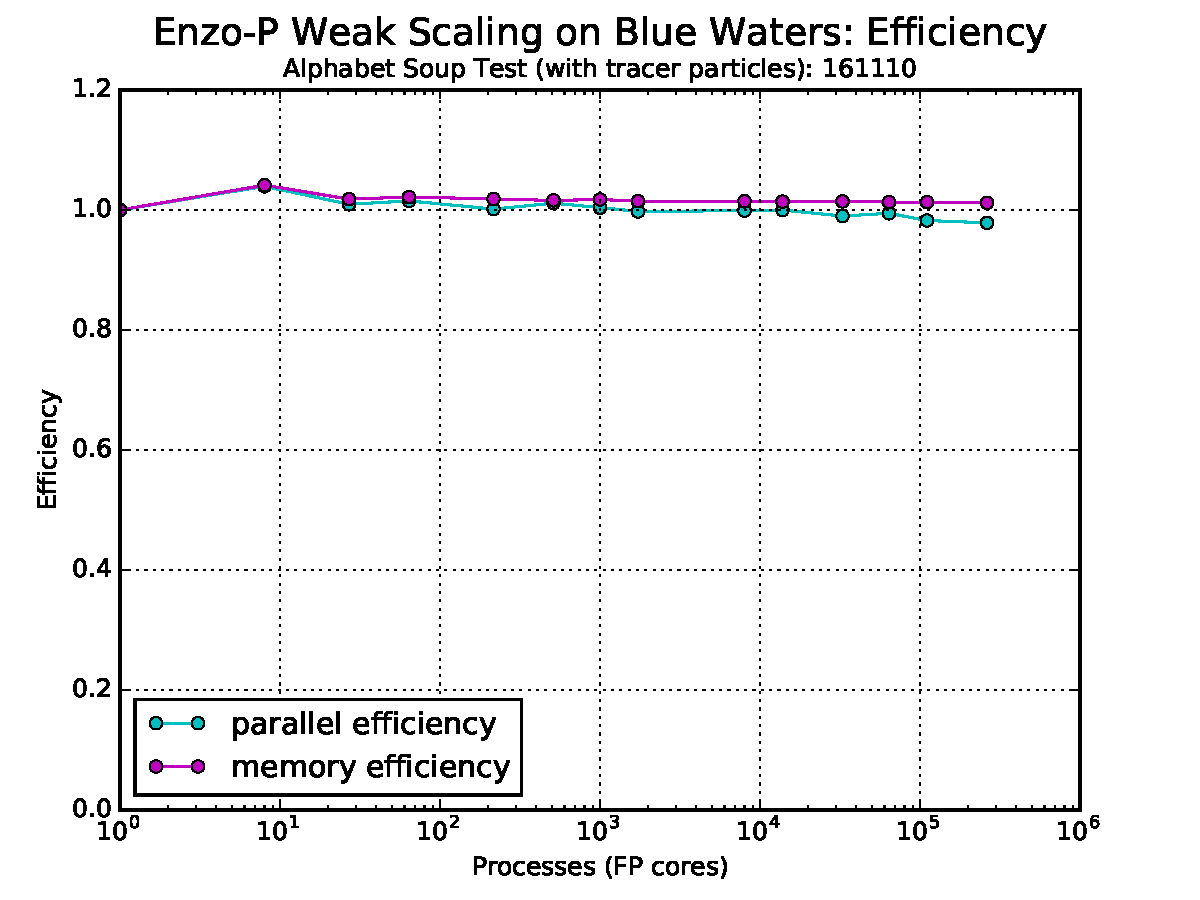
\includegraphics[width=2.0in]{scaling-efficiency-161110.pdf}
    \end{minipage} \ 
      \begin{minipage}{2in}
    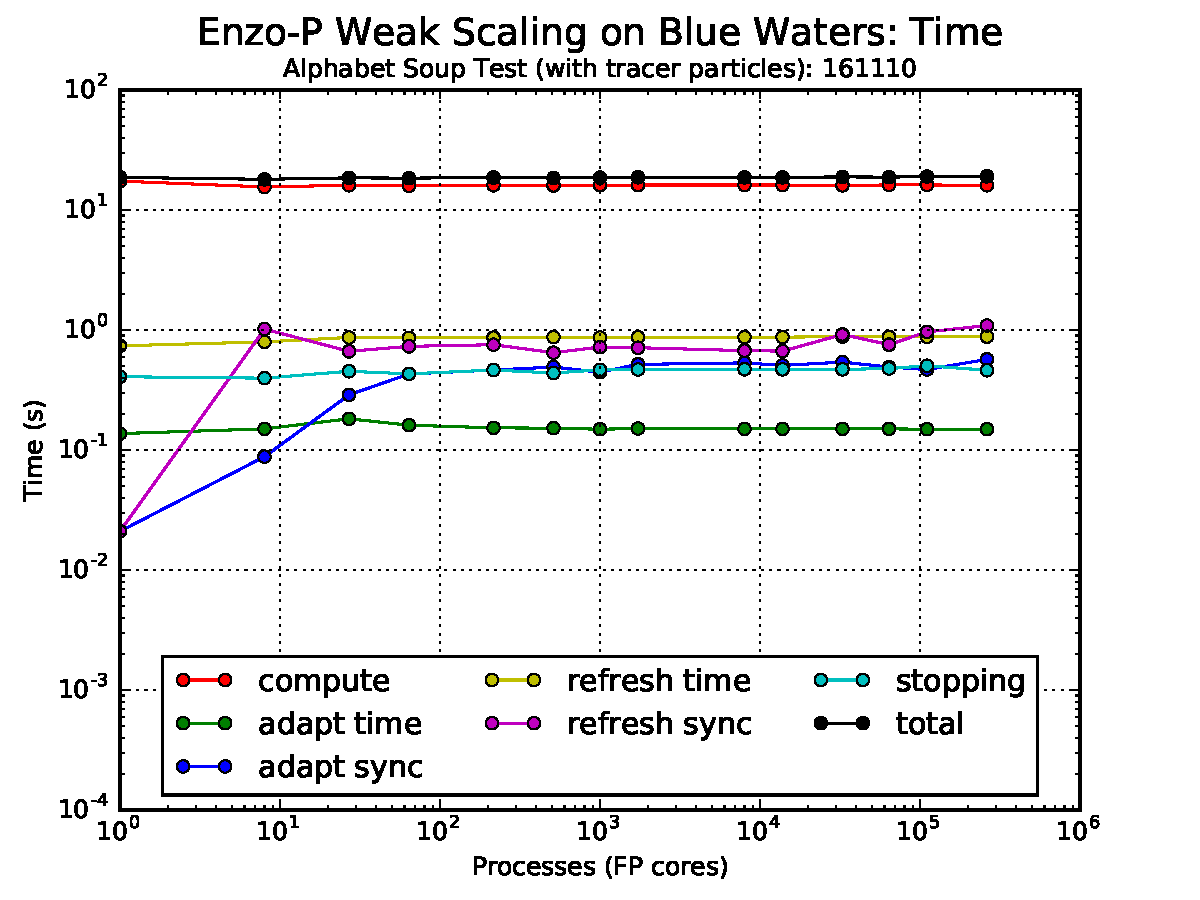
\includegraphics[width=2.0in]{scaling-time-161110.pdf}
    \end{minipage} \\
    \end{center}
  \end{minipage} \\
\end{center}
  
\end{frame}
